%-------------------------
% Usage Examples: Research
%-------------------------

  \subsection*{Research}
    \label{sub:research}

    Often, a disproportionately large component of research involves dealing with various image data-types, color representations, and file format conversion. scikit-image offers robust tools for converting between image data-types \citep{DirectX,OpenGL,GraphicsGemsI} and to do file input/output (I/O) operations.  Our purpose is to allow investigators to focus their time on research, instead of expending effort on mundane low-level tasks.

    The package includes a number of algorithms with broad applications across image processing research, from computer vision to medical image analysis. We refer the reader to the current API documentation for a full listing of current capabilities\footnote{\url{http://scikit-image.org/docs/dev}, Accessed 2014-03-30}. In this section we illustrate two real-world usage examples of scikit-image in scientific research.

    First, we consider the analysis of a large stack of images, each representing drying droplets containing nanoparticles (see Figure~\ref{fig:cracks}). As the drying proceeds, cracks propagate from the edge of the drop to its center. The aim is to understand crack patterns by collecting statistical information about their positions, as well as their time and order of appearance. To improve the speed at which data is processed, each experiment, constituting an image stack, is automatically analysed without human intervention. The contact line is detected by a circular Hough transform (\texttt{transform.hough\_circle}) providing the drop radius and its center. Then, a smaller concentric circle is drawn (\texttt{draw.circle\_perimeter}) and used as a mask to extract intensity values from the image. Repeating the process on each image in the stack, collected pixels can be assembled to make a space-time diagram. As a result, a complex stack of images is reduced to a single image summarizing the underlying dynamic process.

    \begin{figure}[bht]
      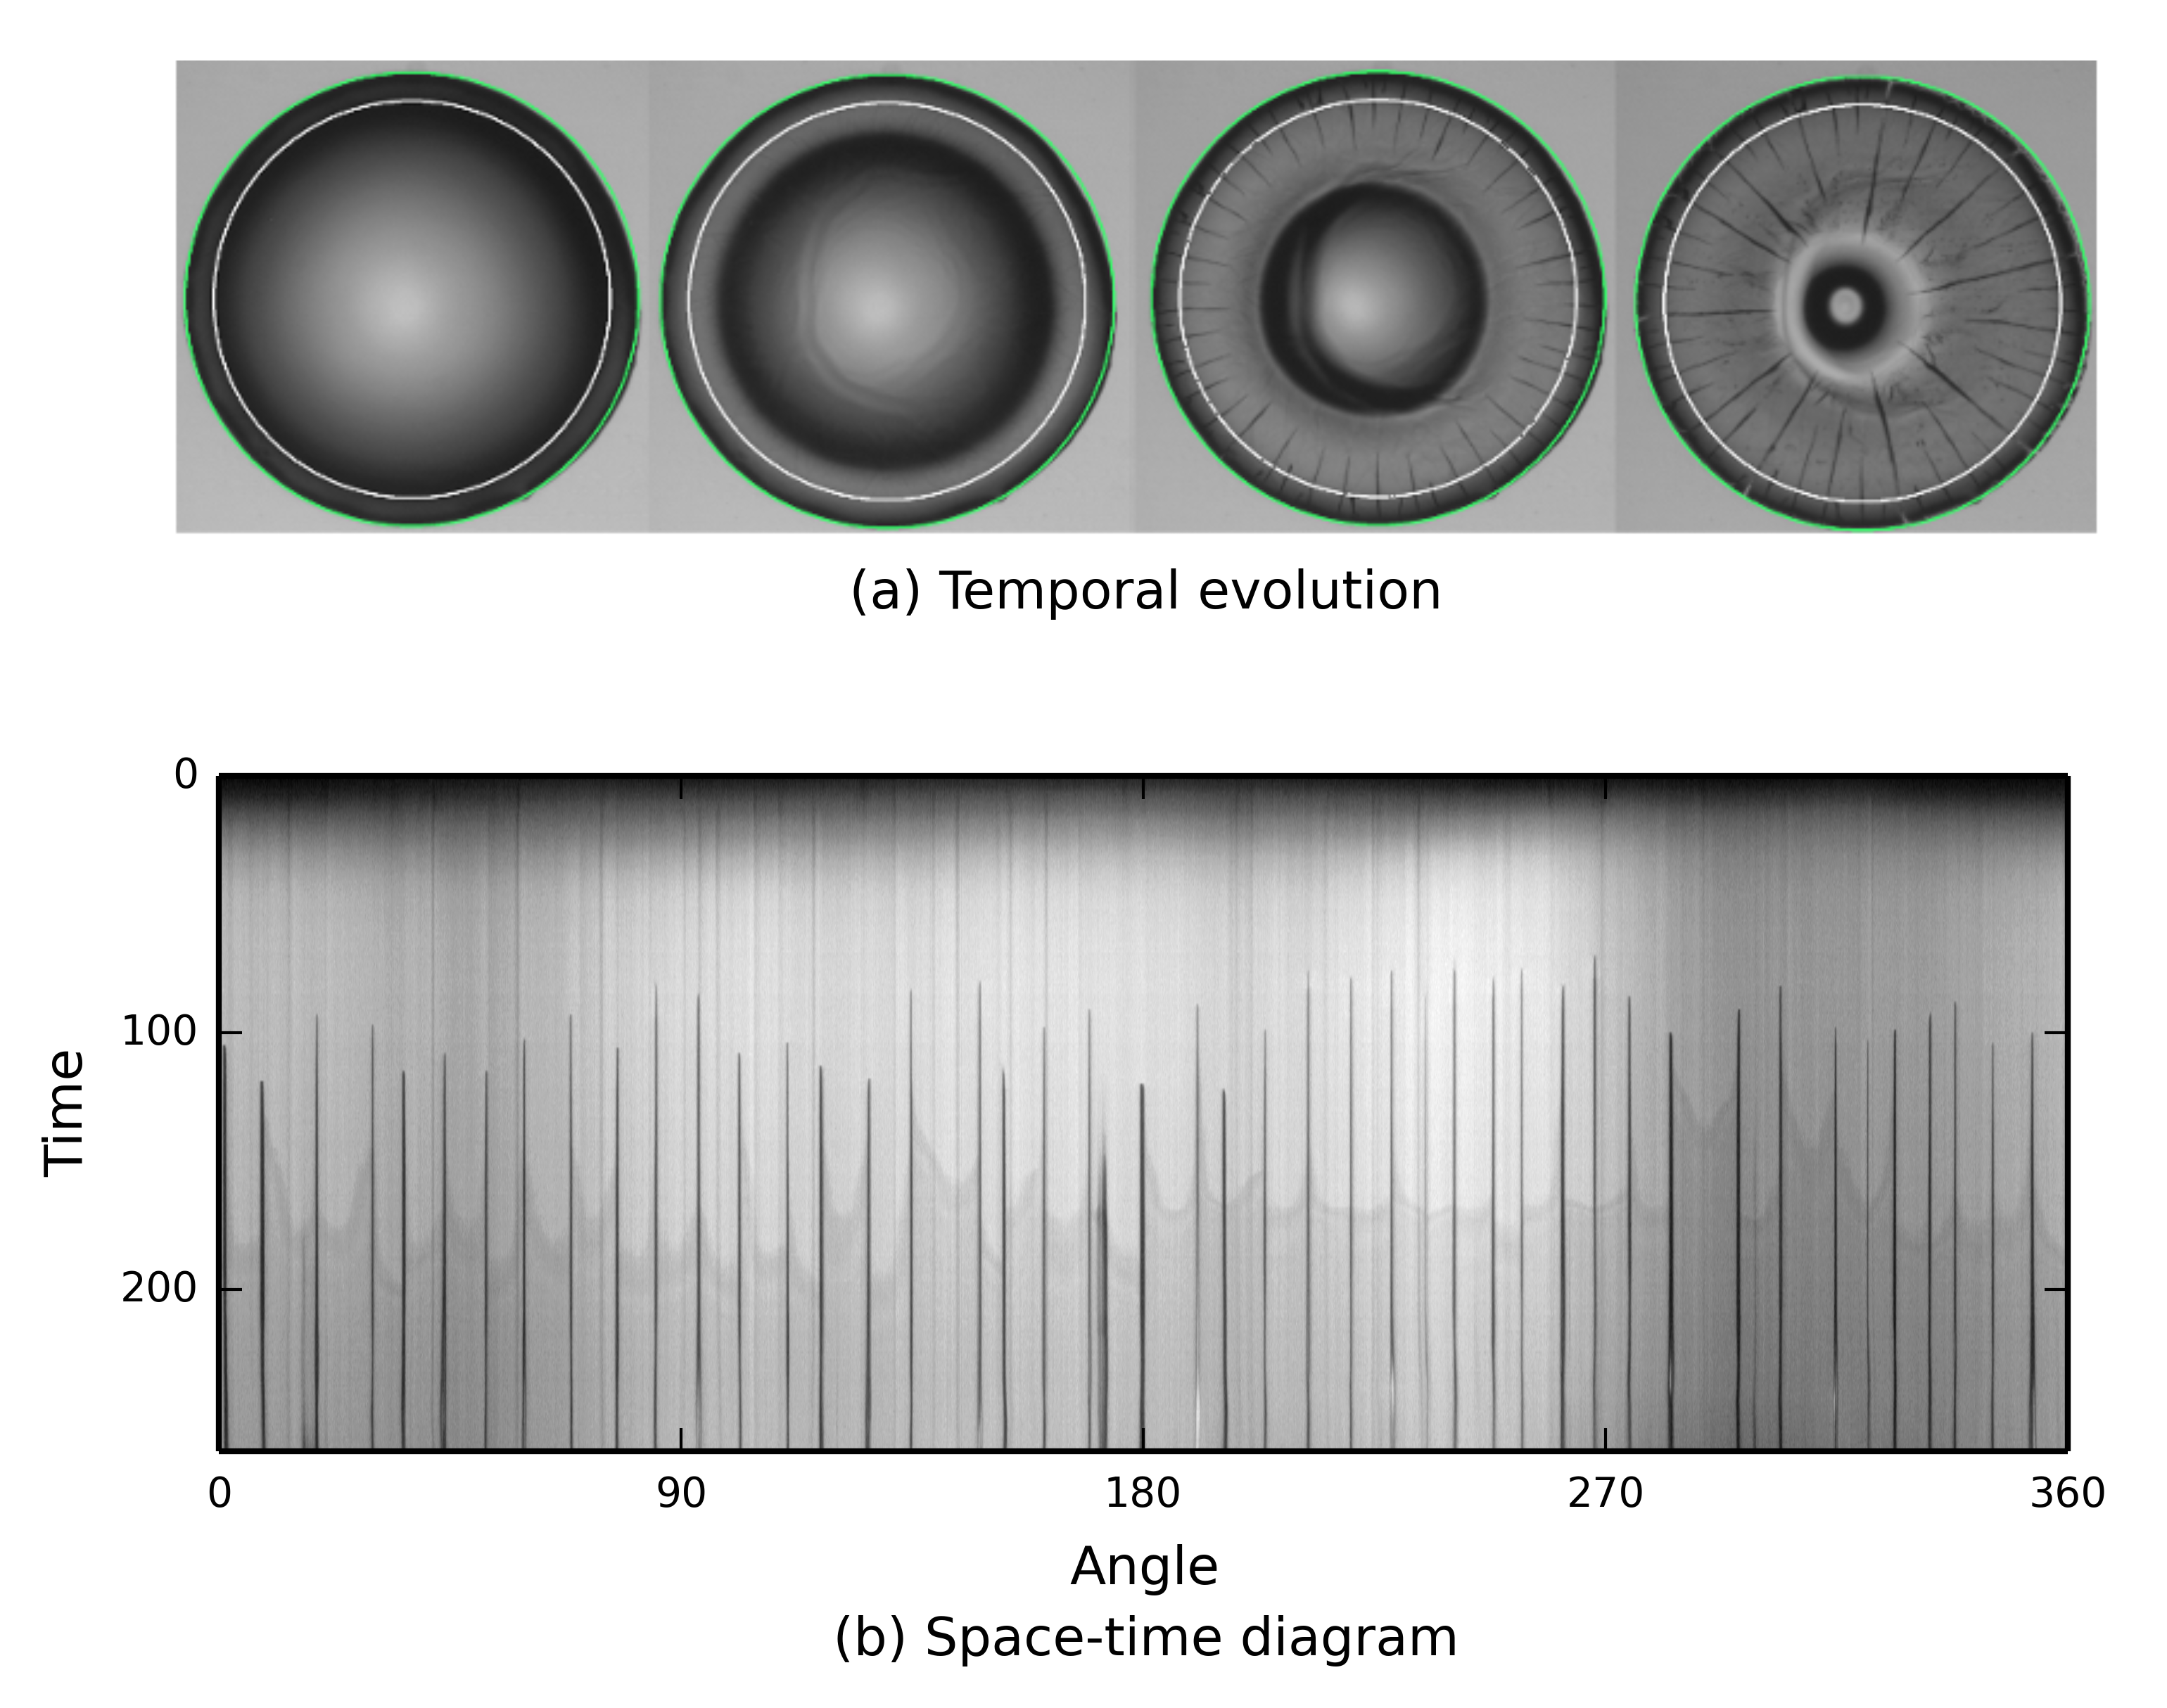
\includegraphics[width=\columnwidth]{fig_cracks.png}

      \caption{scikit-image is used to track the propagation of cracks (black lines) in a drying colloidal droplet. The sequence of pictures shows the temporal evolution of the system with the drop contact line, in green, detected by the Hough transform and the circle, in white, used to extract an annulus of pixel intensities.  The result shown illustrates the angular position of cracks and their time of appearance. \label{fig:cracks}}
    \end{figure}

    Next, in regenerative medicine research, scikit-image is used to monitor the regeneration of spinal cord cells in zebrafish embryos (Figure \ref{fig:profile}). This process has important implications for the treatment of spinal cord injuries in humans \citep{Bhatt04,Thuret06}.

    To understand how spinal cords regenerate in these animals, injured cords are subjected to different treatments. Neuronal precursor cells (labeled green in Figure \ref{fig:profile}, left panel) are normally uniformly distributed across the spinal cord. At the wound site, they have been removed. We wish to monitor the arrival of new cells at the wound site over time. In Figure \ref{fig:profile}, we see an embryo two days after wounding, with precursor cells beginning to move back into the wound site (the site of minimum fluorescence). The \texttt{measure.profile\_line} function measures the fluorescence along the cord, directly proportional to the number of cells. We can thus monitor the recovery process and determine which treatments prevent or accelerate recovery.

    \begin{figure*}[bht]

      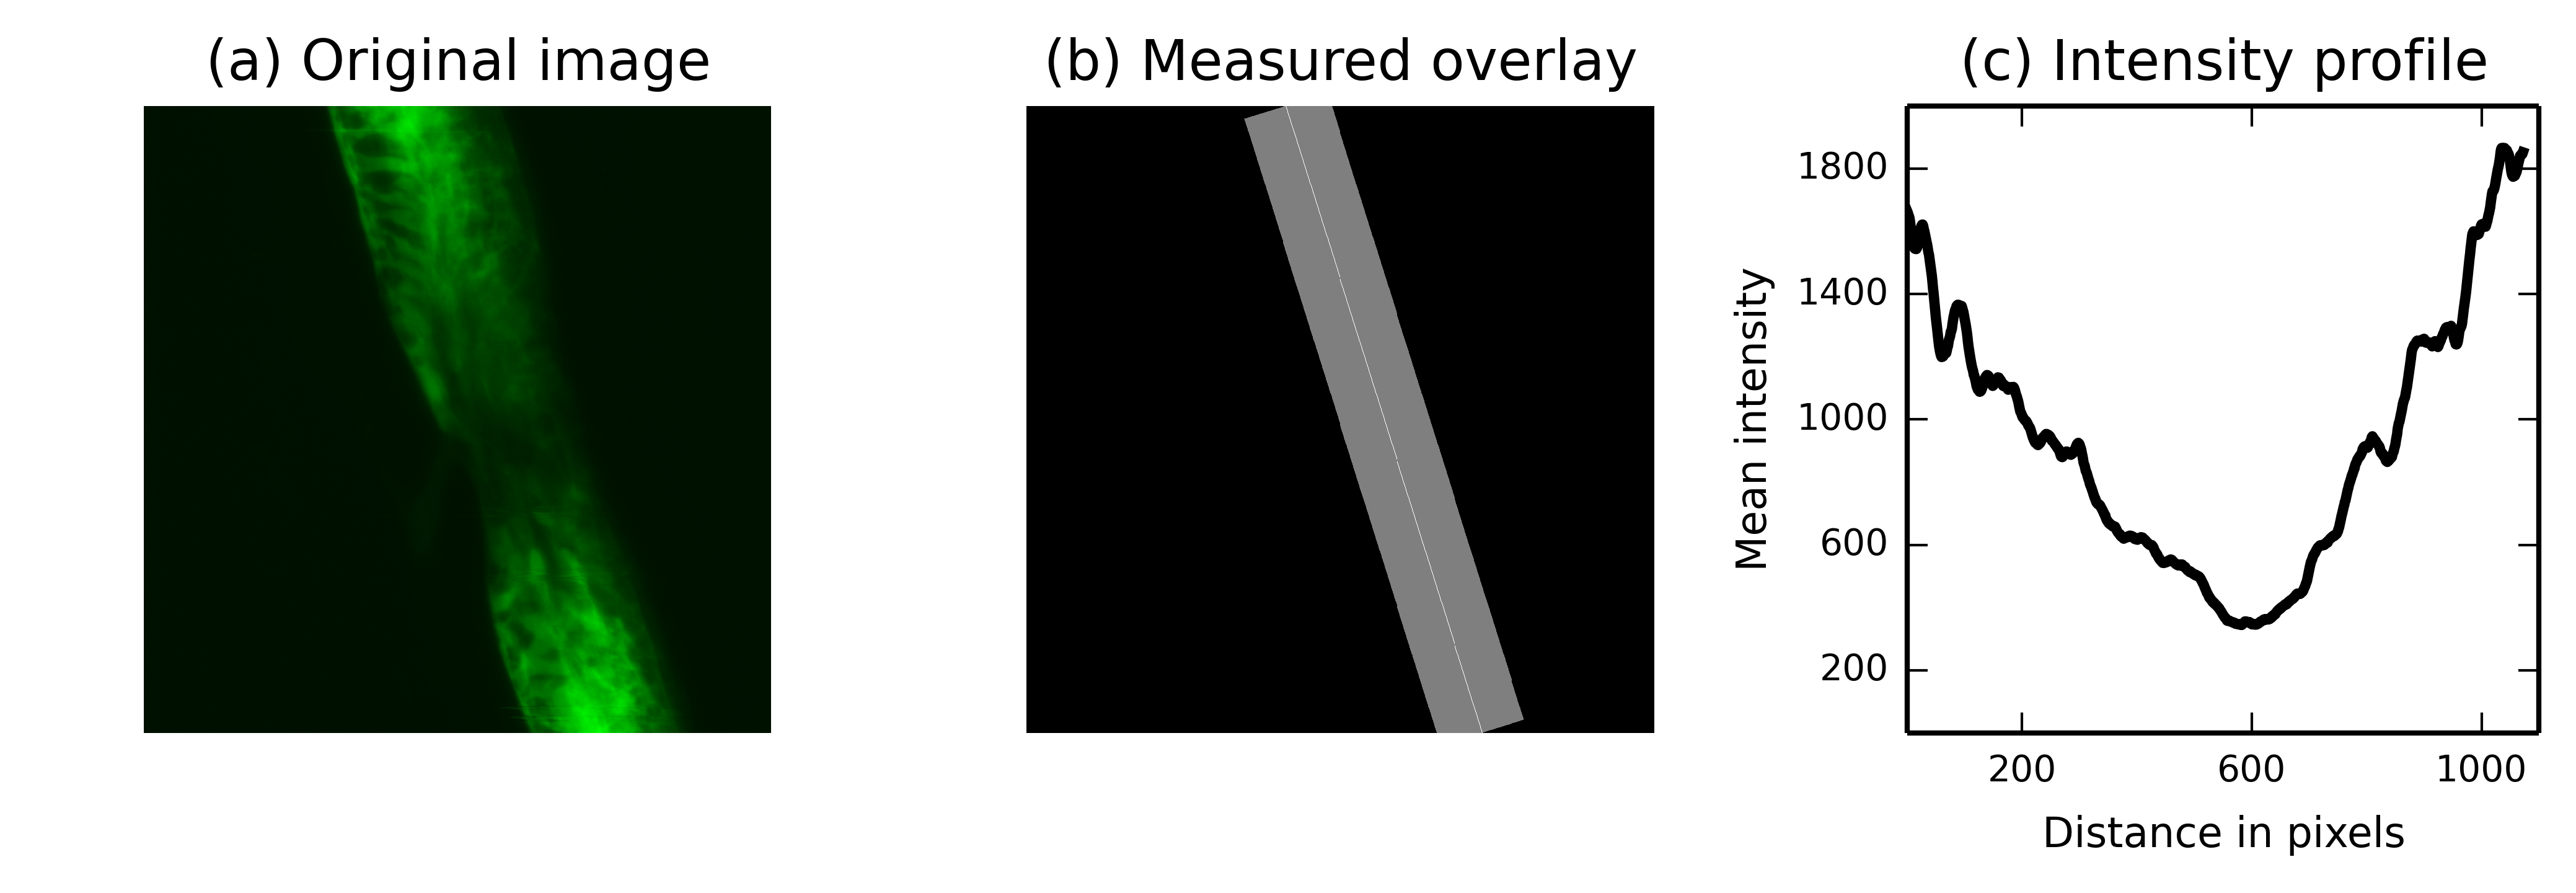
\includegraphics[width=\columnwidth]{fig-lesion.png}

      \caption{The \texttt{measure.profile\_line} function being used to track recovery in spinal cord injuries. (a): an image of fluorescently-labeled nerve cells in an injured zebrafish embryo. (b): the automatically determined region of interest. The SciPy library was used to determine the region extent \citep{scipy,scipylib}, and functions from the scikit-image \texttt{draw} module were used to draw it. (c): the image intensity along the line of interest, averaged over the displayed width. \label{fig:profile}}
    \end{figure*}
